\documentclass{RPI-SIW}

% Load any necessary packages here
\usepackage[OT1]{fontenc}
\usepackage{graphicx,xcolor}
\usepackage{amsmath}
\usepackage{amsfonts}
\usepackage{amssymb}
\usepackage{url}
\usepackage{array, makecell}

\graphicspath{{figs/}}

\begin{document}
\title{A NOVEL SURFACE FEATURE NAVIGATION ALGORITHM USING RAY
TRACING}

\author{
	% Author 1
    Chris Gnam\textsuperscript{1},
	Andrew Liounis\textsuperscript{2}\textsuperscript{*},
    Benjamin Ashman\textsuperscript{2},
    Kenneth Getzandanner\textsuperscript{2},
    Joshua Lyzhoft \textsuperscript{2},
    Jeffrey Small \textsuperscript{3},
    Dolan Highsmith \textsuperscript{3},
    Coralie Adam\textsuperscript{4},
    Jason Leonard\textsuperscript{4},
    Peter Antreasian\textsuperscript{4},
    Dante S. Lauretta\textsuperscript{5},
	% First affiliation
	\textsuperscript{1}Department of Mechanical and Aerospace Engineering, University at Buffalo, State University of New York, Amherst, New York, 14260-4400
    \textsuperscript{2}NASA Goddard Spaceflight Center, 8800 Greenbelt Rd., Greenbelt, MD 20771
	% Second affiliation
    \textsuperscript{3}The Aerospace Corporation, 14745 Lee Rd, Chantilly, VA 20151
    \textsuperscript{4}KinetX Space Flight Dynamics Practice, 21 West Easy Street, Simi Valley, CA 93065
    \textsuperscript{5}Lunar and Planetary Laboratory, University of Arizona, 1415 N 6th Ave, Tucson, AZ 85705
	% Email for POC (currently the first author)
    \textsuperscript{*}[andrew.j.liounis@nasa.gov]
}

\event{2\textsuperscript{nd} RPI Space Imaging Workshop. Saratoga Springs, NY. \\ 28-30 October 2019}
\maketitle{}

\MakeAbstract{
    We demonstrate a novel single-bounce ray tracing approach to landmark identification for surface feature-based relative navigation.  \textit{A priori} knowledge of the camera pose and known topographic maps for each landmark are used to render the potentially visible landmarks via ray tracing into the image frame.  These templates are registered with a search region around the predicted location for each landmark in the image, to locate its observed center.  This procedure is applied to images from the OSIRIS-REx Orbital A and Orbital B mission phases, and the results are compared with those obtained via previous landmark identification methods.
}

\section*{Introduction}
The use of optical navigation (OpNav) for landmark tracking is critical for successful operations around small bodies.  Traditional radiometric tracking methods via the Deep Space Network (DSN) are subject to limitations that can have severe impacts to navigation performance for small body missions.  For periods of the year when the Sun-Earth-probe angle is small, Doppler measurements can experience phase scintillation, as the signal passes through the solar corona.  The magnitudes of these effects are highly dependent on solar activity, and can severely degrade the accuracy of Doppler measurements.\cite{dsn_handbook}  In addition, while radiometric measurements have great precision in the radial direction (with respect to Earth), the along-track and cross-track directions do not fare nearly as well. This means that while the radial position may have an error of only a few meters, the cross-track and along-track errors can range from tens to thousands of meters.   This is acceptable for many planetary missions; however, the magnitude of these errors do not depend on the mass of the body the spacecraft is orbiting.\cite{opnav_near_sb}  Position errors of a few hundred meters would be catastrophic for a mission such as OSIRIS-REx, where the Orbital B mission phase had an altitude of less than 700 meters.  Finally, DSN usage is not continuous and requires scheduling around other missions.

Due to these challenges, the use of radiometric measurements alone cannot provide the relative accuracy required to operate in close proximity to small bodies.  In these scenarios, OpNav measurements can be used to directly relate the spacecraft state to the target surface.  Combining OpNav measurements with DSN measurements, as well as laser altimetry (when available), can be used to not only estimate the spacecraft pose (attitude and position), but also geophysical parameters of the central body such as spin axis/rates, shape model scale, and gravity field coefficients.

The use of landmark-based surface feature navigation has been used to great success in missions such as Hayabusa\cite{hayabusa} and Rosetta\cite{rosetta}, which visited the asteroid Itokawa and the comet  67P/Churyumov Gerasimenko respectively.  The current state-of-the-art approach to landmark-based relative navigation is the stereophotoclinometry (SPC) program developed by Dr. Robert Gaskell of the Planetary Sciences Institute (PSI).  The performance of SPC has been studied extensively;\cite{spc_sensitiviy} however, there are some limitations in its methodology which we will explore.

We propose a novel algorithm as an alternative to SPC's landmark identification, which aims to overcome some of the limitations faced by SPC.  In this paper we will be exploring the details of our new implementation, and comparing its performance with SPC through a variety of methods.  We will also demonstrate the operational performance of this new methodology using navigation images from the OSIRIS-REx mission.

% ====================================================
%     SPC Background
% ====================================================
\section*{Background of SPC Software}
SPC has been used for shape model determination and landmark identification for multiple small body missions.\cite{gaskell_nav_overview}  We will be focusing on SPC's landmark identification functionality, as that is the feature for which our new algorithm provides an alternative.

SPC identifies landmarks via a multi-step process.  First, the expected locations of potentially visible landmarks are calculated using \textit{a priori} state knowledge of the spacecraft.  These locations are then used alongside pre-constructed topographic maps for each landmark (called \textit{maplets}) to generate a \textit{predicted image}.  Next, the illumination values from the image taken by the spacecraft are projected onto the maplet surface creating an \textit{extracted image}.  Finally, image registration is performed between the predicted and extracted images, providing the landmark's precise location in the image.  This process can be repeated for multiple landmarks, and their pixel locations can then be used (potentially alongside other measurement types) to perform orbit determination.

\begin{figure}[h]
	\centering
	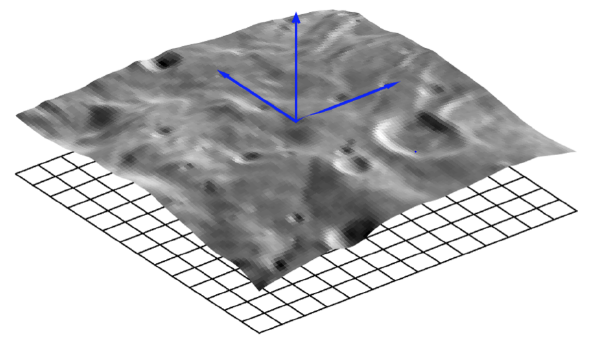
\includegraphics[width=\columnwidth]{spc_maplet.png}
	\caption{Illustration of a \textit{maplet}.  Recall that a \textit{landmark} is a specific point on the surface of the body whose location can be used as a tie point in navigation.  The \textit{maplet} is the topography for the corresponding region around a landmark.}
	\label{figs::maplet}
\end{figure}

\subsection*{Generating the Predicted Image}
In order to generate a predicted image, the intensity of the light reflected off of the maplet surface and into the camera must be precisely modeled.  The intensity of the reflected light depends on the intensity of the incoming light, as well as the directions of both the incident and reflected light, and the surface albedo at the point of reflection.  The phase angle (the angle between the incident light rays and reflected light rays) is also used in some models, including the one presented here.  Functions that model reflections like this are known as Bidirectional Reflectance Distribution Functions (BRDFs).

While many BRDFs exist, many are not physically accurate enough for our purposes (such as the Lambertian BRDF, which models a perfectly matte surface); the way in which these values relate is highly dependent on the specific material, surface roughness, and microstructure.

McEwen proposed a BRDF based on lunar surface data that is well suited for many planetary applications.\cite{mcewen}  SPC utilizes a simple combination of the Lambertian and Lommel-Seeliger reflectance models, as they approximate McEwen's BRDF well.\cite{gaskell_nav_overview}  This illumination model is shown in Eq.~\eqref{eq::mcewen}

\begin{equation}
	\label{eq::mcewen}
	I_k = a_k \left((1-\beta)\cos{(i_k)} + \beta \frac{\cos{(i_k)}}{\cos{(i_k)} + \cos{(r_k)}}\right)
\end{equation}
where for every point $k$, $I$ is the illumination, $a$ is the albedo, $i$ is the incident angle, $r$ is the reflected angle, and $\beta = \exp{(-\alpha/\alpha_0})$ is a weighting term between the Lambertian and Lommel-Seeliger reflectance models (where $\alpha$ is the phase angle in degrees, and $\alpha_0 = 60$).  If we let $\hat{r}_m$ be the vector from the reflection point to the spacecraft sensor, $\hat{s}_m$ be the vector from the reflection point to the Sun, and $\hat{n}$ be the unit normal at the reflection point, then we can easily calculate the values required to evaluate Eq.~\eqref{eq::mcewen}.
\begin{align*}
	\cos{(i_k)} &= \hat{n}_k^T \hat{s}_m \\
	\cos{(r_k)} &= \hat{n}_k^T \hat{r}_m \\
	\alpha &= \cos^{-1}{\left(\hat{s}_m^T \hat{r}_m \right)}
\end{align*}

\begin{figure}[h]
	\centering
	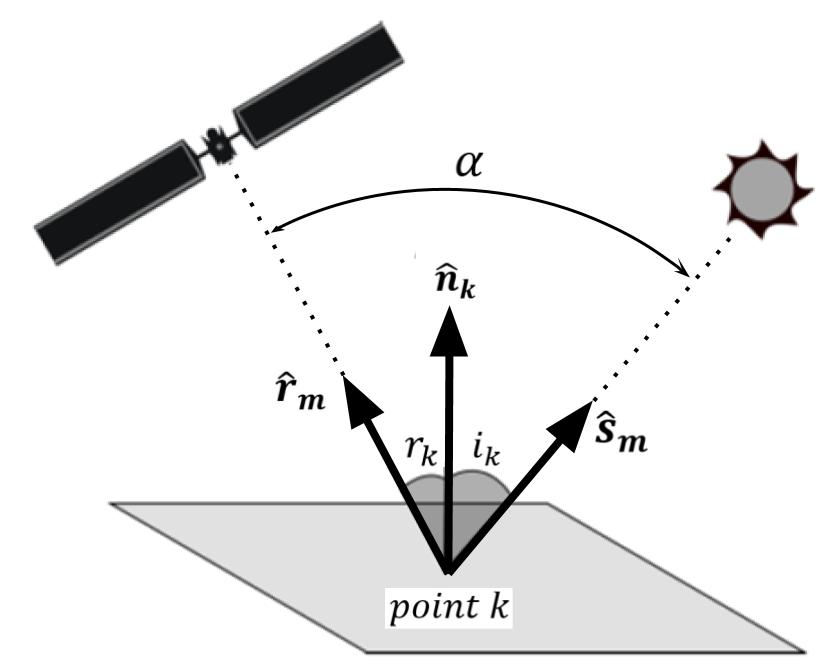
\includegraphics[width=\columnwidth]{brdf.jpg}
	\caption{The geometry used in computing illumination from a BRDF.}
	\label{figs::brdf}
\end{figure}

Using this method along with a known maplet topography (which must be previously constructed via some other method), the surface illumination can be calculated giving a \textit{predicted image}.  It is important to note that the predicted image corresponds directly to the maplet itself.  The calculated intensities for each point on the maplet are not  projected back into the camera frame, but rather remain locked to the maplet surface where later correlation with the extracted image will take place.

Finally, once all of the illumination values are calculated, the entire predicted image is scaled such that the average illumination of the predicted image equals the average illumination of the extracted image.  This aids in the accuracy of the correlation step.

\begin{figure}[h]
	\centering
	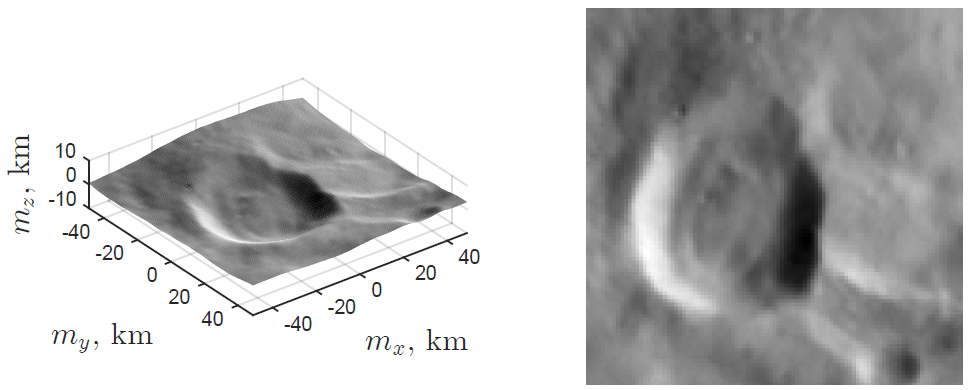
\includegraphics[width=\columnwidth]{predicted_image.png}
	\caption{An example of the illuminated maplet topography (left) and corresponding predicted image (right).  ($m_x$, $m_y$, and $m_z$ correspond to the basis axes of the maplet frame.)}
	\label{figs::predicted}
\end{figure}

\subsection*{Generating the Extracted Image}
Generating the extracted image is a far more complicated process than producing the predicted image.  Because of this, we will not be fully describing every step used to generate an extracted image as implemented by SPC, but will rather focus on the conceptual steps, so as to clearly indicate how our proposed methodology differs.  

The image extraction procedure can be broken down into two fundamental steps: projection onto the maplet topography, and applying the ``extraction filter''.  The fundamental goal of the extracted image is to represent the illumination data captured by the spacecraft camera on the maplet topography itself so that it can be correlated with the predicted image.

\subsection*{Projection onto Maplet Topography}
The first step in image extraction is to project the illumination data onto the maplet topography.  To do this, the correspondences between the expected location of the landmark in the image frame and the location of the landmark in the asteroid-fixed frame are determined.  Because the asteroid-fixed locations of all the landmarks are known (since we are using a pre-constructed shape model), we only need to calculate the expected image frame location of each landmark.  This is done by using an \textit{a priori} estimate of the spacecraft pose and mapping the asteroid-fixed locations through the Owen camera model\cite{owen}.  This is done not just for the landmark locations, but for all the points contained in the landmark's corresponding maplet topography. 

Once all of the points from the maplet topography have been mapped into the image frame, the corresponding illumination values from the image can be projected onto the maplet grid.  In the case where each cell of the maplet grid is smaller than the pixels of the image, then bi-linear interpolation is used to calculate the intensity at a particular cell.  If, however, each cell of the maplet grid is larger than the pixels of the image, then each pixel contained inside a particular cell are averaged to obtain the illumination for that particular cell.

\subsection*{Extraction Filter}
The use of interpolation in the previous step may have assigned illumination values to maplet grid cells that could not possibly be illuminated based on topography of the maplet.  For example, points of the maplet on the inside lip of a crater may not be able to see the Sun, or points over the horizon may not be in sight of the camera.  However, these points may have illumination values assigned to them in the previous projection step due to sensor noise or misalignment errors prior to the interpolation.  Such points must have their illumination values zeroed out in order to perform correlation with the predicted image.

The extraction filter uses both the incidence vector and the reflection vector (shown previously in Fig.~\ref{figs::brdf}) in order to calculate which maplet points should be illuminated.  If the angle between the local unit normal and either of these vectors is greater than $90^{\circ}$, then that point cannot possibly be both illuminated and seen by our camera.  In addition, a cursory check analogous to ray tracing is performed to identify whether any other part of the maplet's topography occludes the current point.  For this, steps are taken along the reflection vector, and each cell crossed by the vector is tested to see if that cell's height is greater than the vector's current height.  If it is, then that cell occludes the point of reflection and so it must be in shadow.  If either of the criteria here are met, then the cell of interest on the maplet is zeroed.  These points are then ignored in the final correlation.

\subsection*{Image Registration}
The previous steps would have likely resulted in many identified maplets.  Stricter constraints can be enforced to remove maplets that are at undesirable orientations or maplets where large amounts of the topography are in shadow.  Once this is done, correlation-based registration is performed to align the extracted and predicted images.  The expression for correlation is given in Eq.~\eqref{eq::corr}.
\begin{equation} \label{eq::corr}
	C = \frac{\frac{1}{N}\sum_{i=1}^k\sum_{j=1}^k (\mathbf{I}_{p}(i,j)\mathbf{I}_{e}(i,j)) - \mu_{p}\mu_{e}}{(\mu_{p2} - \mu_{p}^2)(\mu_{e2} - \mu_{e}^2)}
\end{equation}
where $N$ is the number of pixels, $i$ and $j$ are pixel coordinates of the image, $I_{p}$ and $I_{e}$ are the intensities of the predicted and extracted images respectively, $\mu_{p}$ and $\mu_{e}$ are the mean intensity values for the predicted and extracted images respectively, and $\mu_{p2}$ and $\mu_{e2}$ are the means of the squared intensity values for the predicted and extracted images respectively.

The projected illumination values in the extracted image are shifted around and this correlation process repeated.  This produces a correlation surface, the peak of which represents the best sub-pixel estimate of the landmark location.  Because the camera pose is based on \textit{a priori} state knowledge, any errors in the pose would lead to errors in the predicted and extracted images, that would lead to reduced correlation scores and potentially some landmarks failing to be identified.  Because of this, once all the predicted landmarks are found, a Perspective-n-Point (PnP) solver is run to adjust the camera pose used for generating the predicted and extracted image.  This enables the entire process to be repeated with improved accuracy.\cite{opnav_near_sb}

\begin{figure}[h]
	\centering
	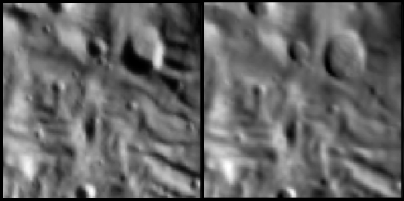
\includegraphics[width=\columnwidth]{spc_sample.png}
	\caption{An extracted image (left) is compared with the corresponding predicted image (right).  Shadows are far more pronounced in the extracted image.}
	\label{figs::sample}
\end{figure}

\subsection*{Potential Weaknesses}
There are several weaknesses associated with this method, however.  First, only the slope of the terrain is considered for illuminating the maplet in the predicted image.  This does not capture shadows in the scene, which are valuable pieces of information.  (The lack of shadows is clear in the predicted image in Fig.~\ref{figs::sample}.)  Further, the extracted image specifically attempts to have shadows ignored from correlation.

In addition, because the image brightness data is extracted onto the surface, additional information about the maplet is artificially injected into the correlation that was not present in the original image.  This makes it possible to overfit the data, particularly when the landmarks are low resolution, which means that the difference in ground sample distance between the maplet and image is large.

Finally, because the correlation is performed on the maplet itself, the maximum shift that can be retrieved using this method is limited by half the size of the landmark.  
This can make it difficult to perform SPC when the initial error in the \textit{a priori} state is very large, and typically requires registering the entire image to the global shape model first, before attempting surface feature navigation.

% ====================================================
%     Proposed Methodology
% ====================================================
\section*{Proposed New Methodology}
We propose a novel algorithm as an alternative to the SPC method described above.  It aims to overcome some of the limitations discussed for SPC by taking a fundamentally different approach to registering a predicted landmark with the image taken by the spacecraft.  We do this by using a single-bounce ray tracer to render the maplet directly into the image frame, where it is then registered.  The ray tracing algorithm also accurately renders shadows which can then be used in the registration step.  This algorithm can be broken into several primary steps, with some being fundamentally the same as the steps in SPC.  The difference of this proposed method is in how the predicted image (referred to in this section as the \textit{template}) is rendered and registered with the image captured by the spacecraft.

An additional benefit to rendering the template into the image space (where the correlation is then performed) is that the landmark can be potentially identified anywhere in the image.  This is because during the registration process, the rendered template can be shifted to any location in the captured image, and so the maximum allowable shift is limited only by the size of the image.  When correlation is done on the maplet (as is done in SPC), one is limited to a maximum shift that is the size of the maplet.  This can cause issues if \textit{a priori} knowledge of the spacecraft pose is poor.

It is important to remember that this approach is purely for the landmark identification step in the overall surface feature-relative navigation procedure.  This new approach is not for use in actual shape model construction or maplet generation, and assumes that maplets/landmarks have already been created by SPC or some other method.  We will discuss the implications of this in our conclusions section. 

An example of the aligned templates with the image produced by the steps described in this section is shown in Fig.~\ref{fig:sample_template}.
\begin{figure}
	\centering
	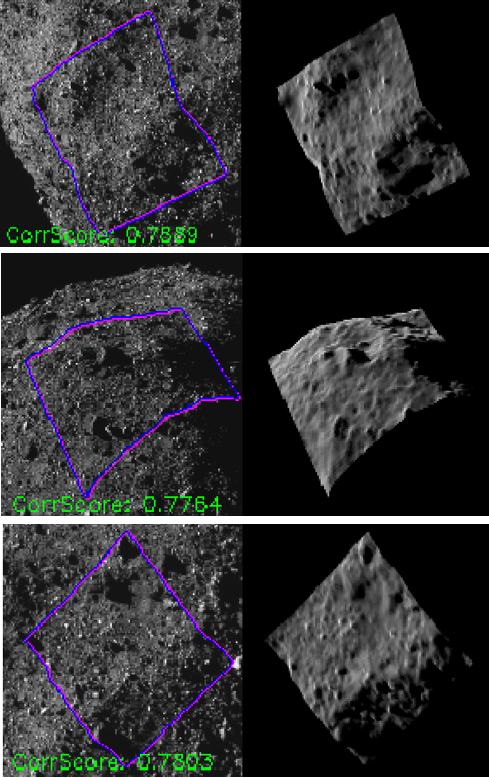
\includegraphics[width=\columnwidth]{figs/sfn_sample2.png}
    \caption{An output from the implementation of the algorithm described in this paper in the Goddard Image Analysis and Navigation Tool (GIANT). \textbf{Left:} A cropped portion of a NavCam 1\cite{tagcams} image of Bennu in Orbital A. \textbf{Right:} The rendered template of a feature observed in the image.  In the cropped image the pink outline is the predicted location while the blue outline is the solved-for location.}
	\label{fig:sample_template}
\end{figure}

\subsection*{Landmark Prediction}
Similar to SPC, potentially visible features are identified using an \textit{a priori} estimate of the camera pose as well as the orientation of the target object. Once these potentially visible landmarks have been identified, they are projected into the camera frame (using a pre-calibrated camera model) to obtain the predicted centers for each.

\subsection*{Template Rendering using Ray Tracing}
The rendering of the landmarks into image templates takes place wholly in the image frame via a ray tracing method.  Ray tracing is a rendering technique which traces light backwards from the camera to a light source.  To do this, rays for each image pixel are traced through a model of the camera and into the scene where they are checked to see if they intersect with any of the topography.  In a single-bounce ray tracer, if the ray strikes a surface, then a new ray is traced from the intersection point to the light source (the Sun in our case).  If the reflected ray intersects with any other part of the topography, then the reflection point is in shadow.  If the reflected ray does not intersect with anything else, then the illumination for that ray (and thus its corresponding pixel in the image frame) is computed.  This process is shown in Fig.~\ref{figs::ray_tracing}.

In our case, the topography data for all identified features are loaded from a feature catalog.  Individual maplets are loaded, and single-bounce ray tracing is performed, where rays are cast through a pre-calibrated model of the camera and intersections with the maplet surface are identified.  The rays are traced back to the Sun, and any additional intersections indicate the point on the maplet is in shadow.  This information is run through an illumination model to fully render the illuminated surface into the image space, as a \textit{template}.  For the purposes of this paper we are using the McEwen BRDF to calculate the surface illumination.\cite{mcewen}
\begin{figure}
	\centering
	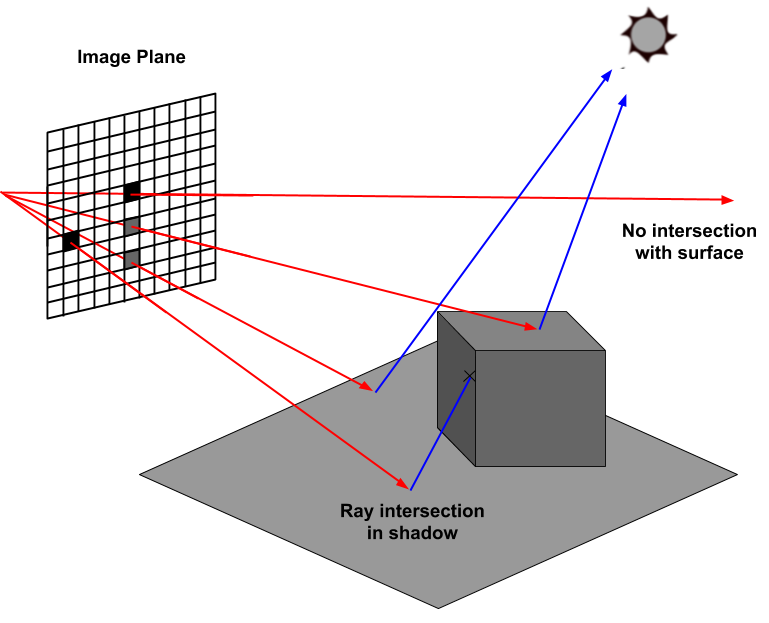
\includegraphics[width=\columnwidth]{ray_tracing.png}
	\caption{The geometry of a single-bounce ray trace for a simple scene.}
	\label{figs::ray_tracing}
\end{figure}

To prevent aliasing, and to improve overall performance of this approach, a technique known as super sampling can be employed.  Super sampling is the technique whereby multiple rays are cast for each pixel, and the calculated intensities for each ray are averaged to produce the overall illumination value of the pixel.  This helps to soften edges and capture sub-pixel variations in a way more representative of the inner workings of a camera, in exchange for increased computational expense.

\subsection*{Cropping and Masking}
Once a rendered template has been produced, the actual image captured by the spacecraft must be appropriately cropped in order to effectively perform the correlation.  In addition to this cropping, two masks are produced from both the original image as well as the rendered template.  First, if none of the rays for a given pixel intersected the maplet, then that pixel is removed from the \textit{intersection mask}.  Additionally, any pixel in the image collected by the spacecraft containing space is identified and added to the \textit{space mask}.  These two masks are then combined with a logical or and used to tell the correlator to include these pixels in the cross-correlation.  This ensures that only actual surface features and space are being correlated, not regions around a feature that were not rendered.  An example of this process is shown below in Fig.~\ref{figs::masks}, for a specific alignment of a template and cropped image location.  Due to the severe overlap of the maplet and space, it is clear that this is not the correct alignment.  This masking process is repeated for every alignment in the image registration process, which is discussed next.
\begin{figure}
	\centering
	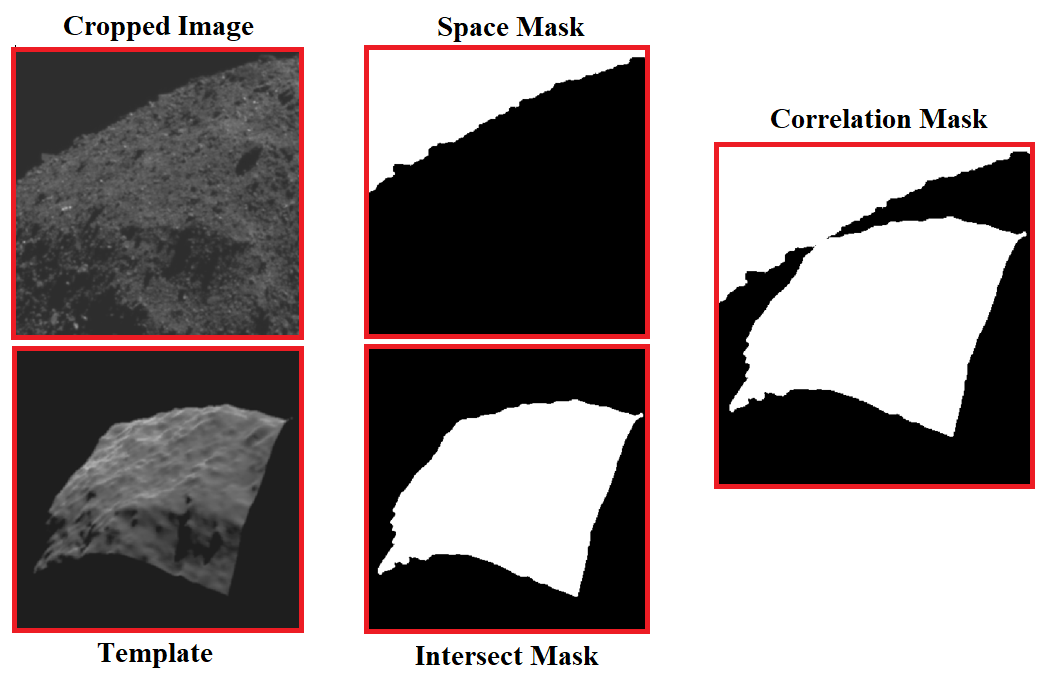
\includegraphics[width=\columnwidth]{figs/masks.png}
	\caption{A diagram showing the generation of the correlation mask by determining a space mask from the cropped image and an intersection mask from the rendered template.  The two masks are combined with a logical or to determine which pixels to include in the computation of the correlation score for this template.}
	\label{figs::masks}
\end{figure}

\subsection*{Normalized Cross Correlation}
Using the predicted centers for each landmark, a search region is defined around where the landmark is expected to be in the image.  The previously rendered templates are then registered with this search region to estimate where the landmark is in the region, and thus its location in the image as a whole.  The registration is done using the standard normalized cross-correlation, with various alignments of the template in the search region which creates a correlation surface.  A least-squares algorithm is then used to fit a paraboloid to the correlation surface.  This allows for sub-pixel accuracy in estimating the peak of the correlation surface, which corresponds to the estimated center of the landmark in the search region.

\subsection*{PnP and Measurement Refinement}
Because the camera pose is based on \textit{a priori} state knowledge, any errors in the pose would lead to errors in rendering the templates, which would thus decrease correlation scores and potentially lead to some landmarks failing to be identified.  Therefore, once all landmark locations have been identified in the image, a PnP solver can be run to adjust the camera pose.  The templates are then re-rendered, and the image registration process is repeated with the new templates, allowing for more precise landmark locations to be estimated.

% ====================================================
%     SPC Comparison
% ====================================================
\section*{Comparison with SPC}
While the landmark location prediction and PnP steps between both methods are mostly the same, there are some substantial differences as we previously discussed.  These have been organized into Table \ref{tab:compare} to provide an easy comparison between the two methods.
\renewcommand{\arraystretch}{2}
\begin{table*}[tb]
	\centering
	\caption{A condensed comparison between SPC and the present methodology.}
    \begin{tabular}{c|m{0.43\textwidth}m{0.43\textwidth}}
        \hline\hline
        & SPC & Present Methodology\\
        \hline
        \rotatebox[origin=c]{90}{Prediction} & A predicted image is created by using the McEwen BRDF to calculate illumination values for every point on the maplet surface. & A template image is rendered into the camera frame via ray tracing.  The McEwen BRDF is then used to calculate illumination values for each pixel in the template.  If the ray does not intersect the maplet, then that pixel is removed from the intersection mask. \\
        \rotatebox[origin=c]{90}{Extraction} & An extracted image is created by projecting the illumination values from the collected image on the maplet surface.  A simple method is then used to identify shadows and obstructed regions. & All of the pixels in the collected image that are of space included in the space mask.  The image is then cropped to only contain the region where the landmark is expected to be for each potential alignment, creating the cropped image.\\
        \rotatebox[origin=c]{90}{Registration} & Cross-correlation between the predicted image and the extracted image takes place on the maplet surface.  Regions where shadows are expected to be, or pixels in the image detected to be in shadow (due to being below a certain threshold), are ignored in the correlation.& Cross-correlation between the template and cropped image takes place in the image frame.  The intersection mask and space mask are combined so that only relevant portions of both the template and image are correlated.  Importantly, shadows are included in the computation of the correlation surface.\\
        \rotatebox[origin=c]{90}{Registration} \rotatebox[origin=c]{90}{Location} & Because the cross-correlation takes place on the maplet surface, the amount that the predicted image can be shifted by is limited by the size of the template. & Because the cross-correlation takes place in the image frame, the only limit on shifting the template is the size of the image itself.  This can be beneficial if \textit{a priori} knowledge in the spacecraft pose is poor.\\
        \hline
        \hline
    \end{tabular}
	\label{tab:compare}
\end{table*}

% ====================================================
%     GIANT Implementation
% ====================================================
\section*{Implementation into GIANT}
The Goddard Image Analysis and Navigation Tool (GIANT) provides a suite of python tools which enable easy camera calibration as well as processing of images for both stellar OpNav and relative OpNav. The structure and basic functionality of GIANT is explored by A. Liounis (2019).\cite{giant}  The method proposed here was implemented as the \textbf{SFN} module in the \textbf{relnav} package, and now provides surface feature navigation capabilities to GIANT.

\subsection*{k-d tree for ray tracing optimization}
Ray tracing requires testing for intersections between a ray and the given topography.  In many implementations of ray tracing, the topography is first tesselated into a triangular mesh, as there are many fast algorithms for testing triangle-ray intersections \cite{triangle_ray}.  As the topography increases in detail (and thus complexity), the number of triangles increases.  Checking if a ray intersects with every triangle can therefore be prohibitively expensive.  Because of this, it is desirable to reduce the number of triangles that must be checked for each ray.

We accomplished this by implementing a k-dimensional search tree (k-d tree), which is a space-partitioning data structure.  The space containing our topography is recursively divided in half (each split producing a new node in a binary search tree).  Each split is then defined by an axis-aligned bounding box.  This process continues until a hand-tuned number of triangles remain in each bounding box.  These final bounding boxes are known as the \textit{leaves} of the search tree.

This method of organizing the topography means that we no longer need to test the ray for intersection with every triangle in the scene.  The ray is first tested against the first two bounding boxes (which each represent half of our scene).  If the ray does not intersect either of them, no further checks are needed.  If the ray does intersect one of them (or both of them), further checks are done on the sub-bounding boxes for each.  This process is repeatedly recursively until either no intersection is found, or until a leaf is reached, at which point the ray is tested against only a small number of triangles.  Because the intersection check between a ray and an axis-aligned bounding box is extremely computationally efficient, and because the number of bounding boxes that need to be checked is much smaller than the total number of triangles in the shape model, this technique allows for dramatic improvement in the computational efficiency of the ray trace. 
While constructing the tree is somewhat expensive, it only needs to be done once for every model and is then stored for future use.

% ====================================================
%     OSIRIS-REx Orbit A Results
% ====================================================
\section*{Processing of OSIRIS-REx Images}
The OSIRIS-REx asteroid sample return mission began proximity operations around near-Earth asteroid Bennu in late 2018.  In January and February of 2019, OSIRIS-REx was in the Orbital A mission phase, where it operated in a frozen terminator orbit around Bennu at altitudes roughly between 1.35 km and 1.85 km.  It was during this period that the navigation team transitioned from centroid-based relative navigation to landmark-based navigation using SPC.

On June 12, 2019, OSIRIS-REx performed a maneuver that decreased its altitude to 680 m above Bennu's surface and entered the Orbital B mission phase.  The decreased altitude allowed the OSIRIS-REx Laser Altimeter (OLA)\cite{ola} to produce a full terrain map, and PolyCam\cite{ocams} to generate a high-resolution global image mosaic.  The Orbital B mission phase lasted until August 2019, at which point the spacecraft ascended to a slightly higher altitude for further science observations.

The navigation images taken by NavCam 1\cite{tagcams} from both of these mission phases were processed using the GIANT SFN implementation, as well as SPC.  These results were then used along with radiometric measurements from the DSN in the GEODYN II precision orbit determination and geodetic parameter estimation program, to perform orbit determination.  The solutions obtained via this process were then compared with the trajectory solutions obtained by KinetX, the prime navigation team.

In each of the following sections (for both Orbital A and B) we show a comparison of the trajectories (both the position and velocity over time) in the Bennu centered RIC frame.  We then show the post-fit residuals for both the SFN and SPC solutions. These results demonstrate that the current implementation of SFN in GIANT performs similarly to SPC.

\subsection*{Orbital A}
\begin{figure}[h]
	\centering
	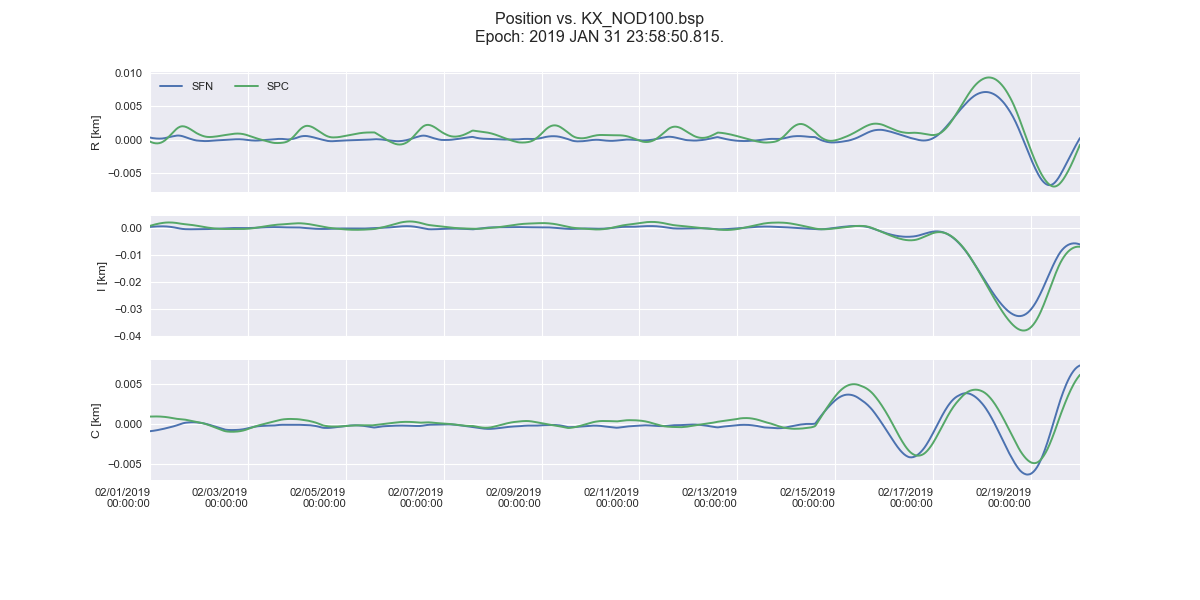
\includegraphics[width=\columnwidth]{orbita_pfig.png}
    \caption{Trajectory position differences in the Bennu radial, in-track, cross-track (RIC) frame during Orbital A.  The comparison is between an orbit determination solution which uses SFN as the source of surface feature observations and the official orbit determination solution produced by KinetX which uses SPC as the source of surface feature observations.}
    \label{fig:oapos}
\end{figure}
\begin{figure}[h]
	\centering
	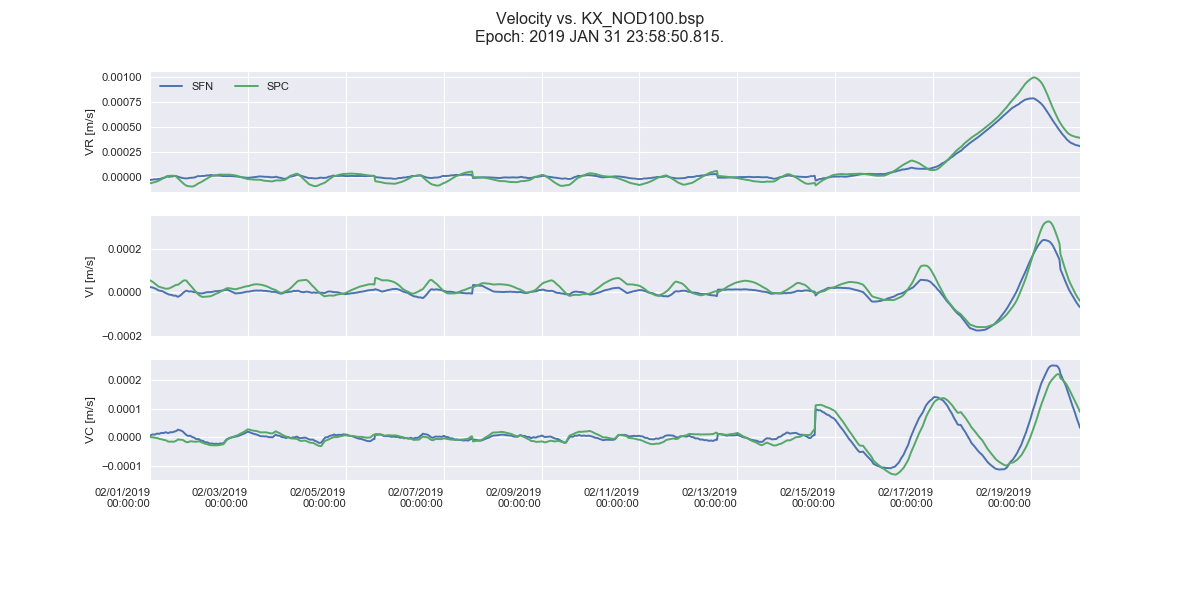
\includegraphics[width=\columnwidth]{orbita_vfig.png}
    \caption{Trajectory velocity differences in the Bennu radial, in-track, cross-track (RIC) frame during Orbital A.  The comparison is between an orbit determination solution which uses SFN as the source of surface feature observations and the official orbit determination solution produced by KinetX which uses SPC as the source of surface feature observations.}
    \label{fig:oavel}
\end{figure}
The trajectories from the SFN and SPC processing match both each other and the KinetX solution quite closely over the period of time when observations were collected, as seen in Figs.~\ref{fig:oapos} and \ref{fig:oavel}.  The oscillations seen at the end of the arcs are due to the data cutoff, at which point no further data are included in the solution and the spacecraft state is based purely on dynamics integration.  This was done to evaluate the prediction performance of each technique.  The SFN data produces a very similar orbit to that estimated using the SPC data, indicating that the method is working at least as well as SPC.

\textbf{OpNav Post-fit Residuals:}
\begin{figure}[h]
	\centering
	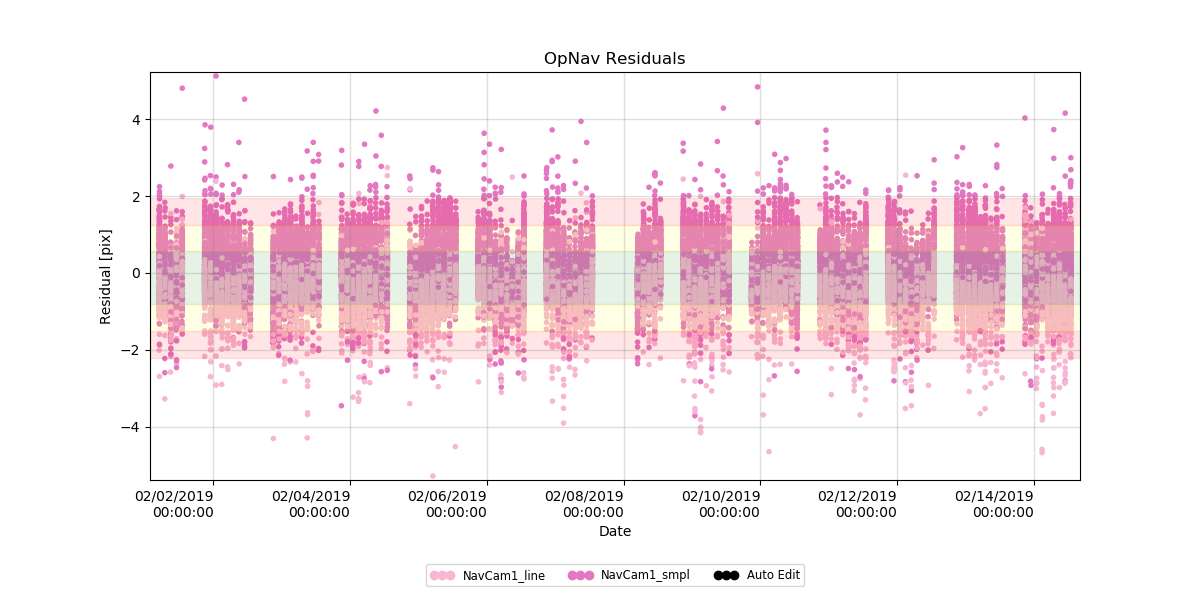
\includegraphics[width=\columnwidth]{orbita_sfn.png}
    \caption{Post fit surface feature navigation residuals from GEODYN using GIANT SFN as the source of surface feature observation in Orbital A.}
    \label{fig:oasfn}
\end{figure}
\begin{figure}[h]
	\centering
	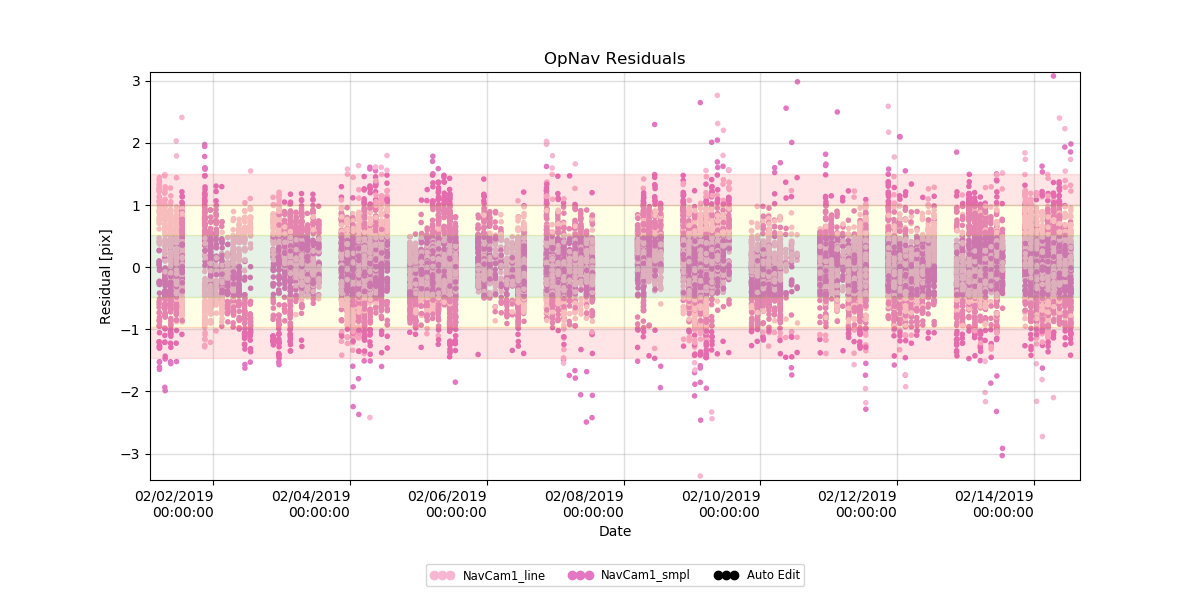
\includegraphics[width=\columnwidth]{orbita_spc.png}
    \caption{Post fit surface feature navigation residuals from GEODYN using SPC as the source of surface feature observation in Orbital A.}
    \label{fig:oaspc}
\end{figure}
Fig.~\ref{fig:oasfn} shows the post-fit residuals of the GIANT SFN observation in the GEODYN OD solution, and Fig.~\ref{fig:oaspc} shows the same but for the SPC Residuals.  The post-fit residuals are similar as should be expected since the fit trajectories are similar.

% \textbf{DSN Residuals:}
% \begin{figure}[h]
% 	\centering
% 	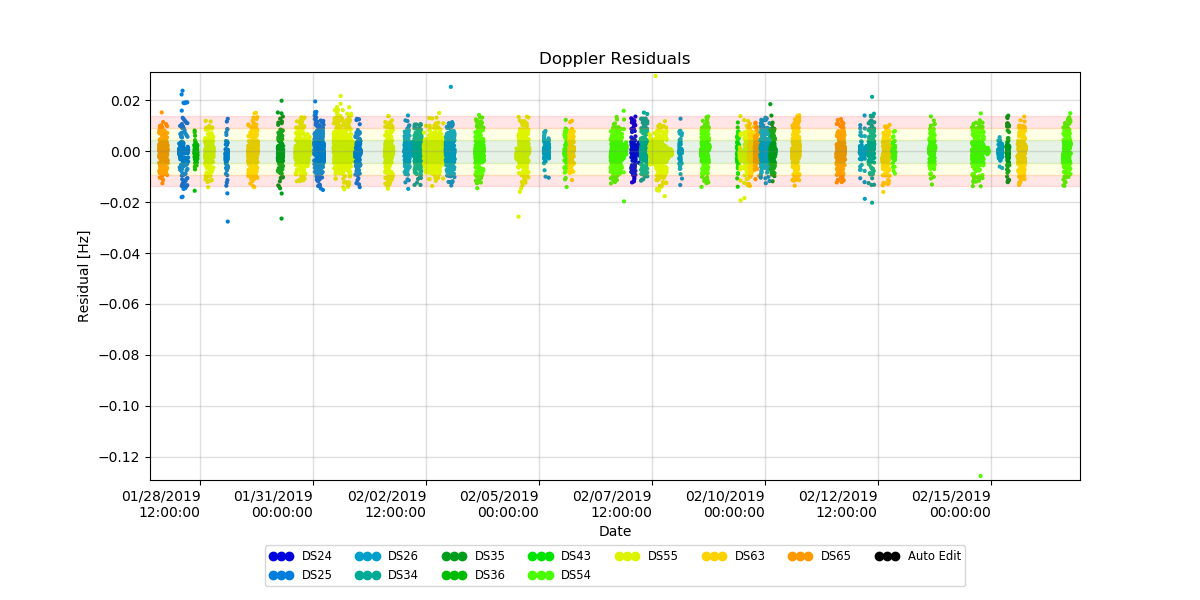
\includegraphics[width=\columnwidth]{orbita_doppler.png}
% \end{figure}
% \vspace{-1cm}
% \begin{figure}[h]
% 	\centering
% 	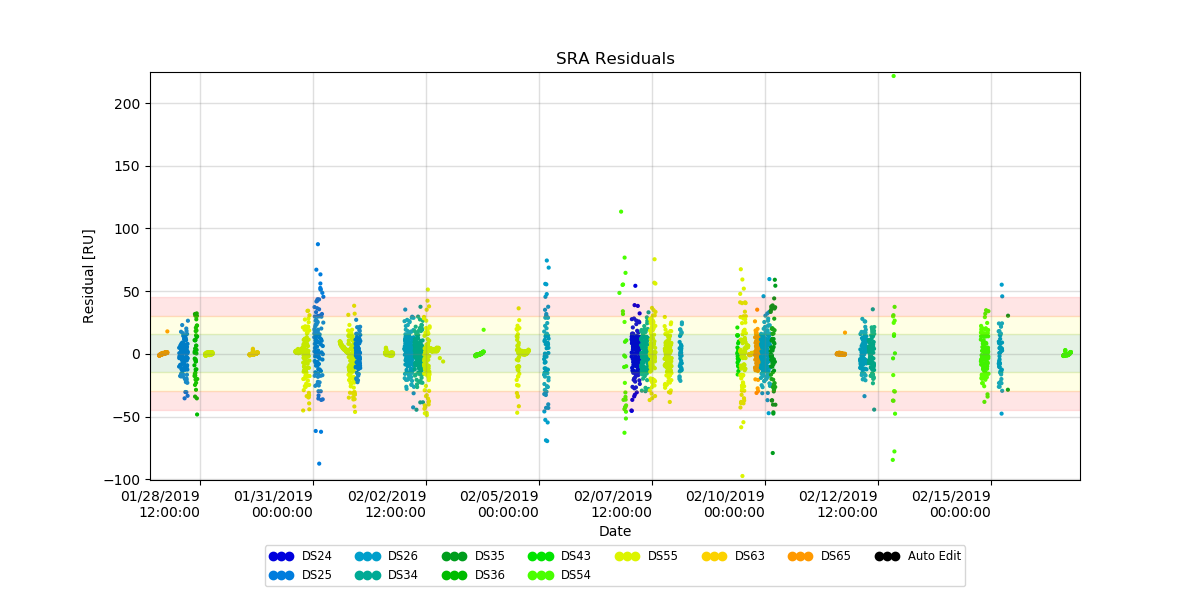
\includegraphics[width=\columnwidth]{orbita_sra.png}
% \end{figure}
% The above plots show the range and doppler post-fit residuals for the SFN solution.  The SPC range and doppler solutions were nearly identical.
% \vfill
% 
% 
% 
% \pagebreak
\subsection*{Orbital B}
\begin{figure}[h]
	\centering
	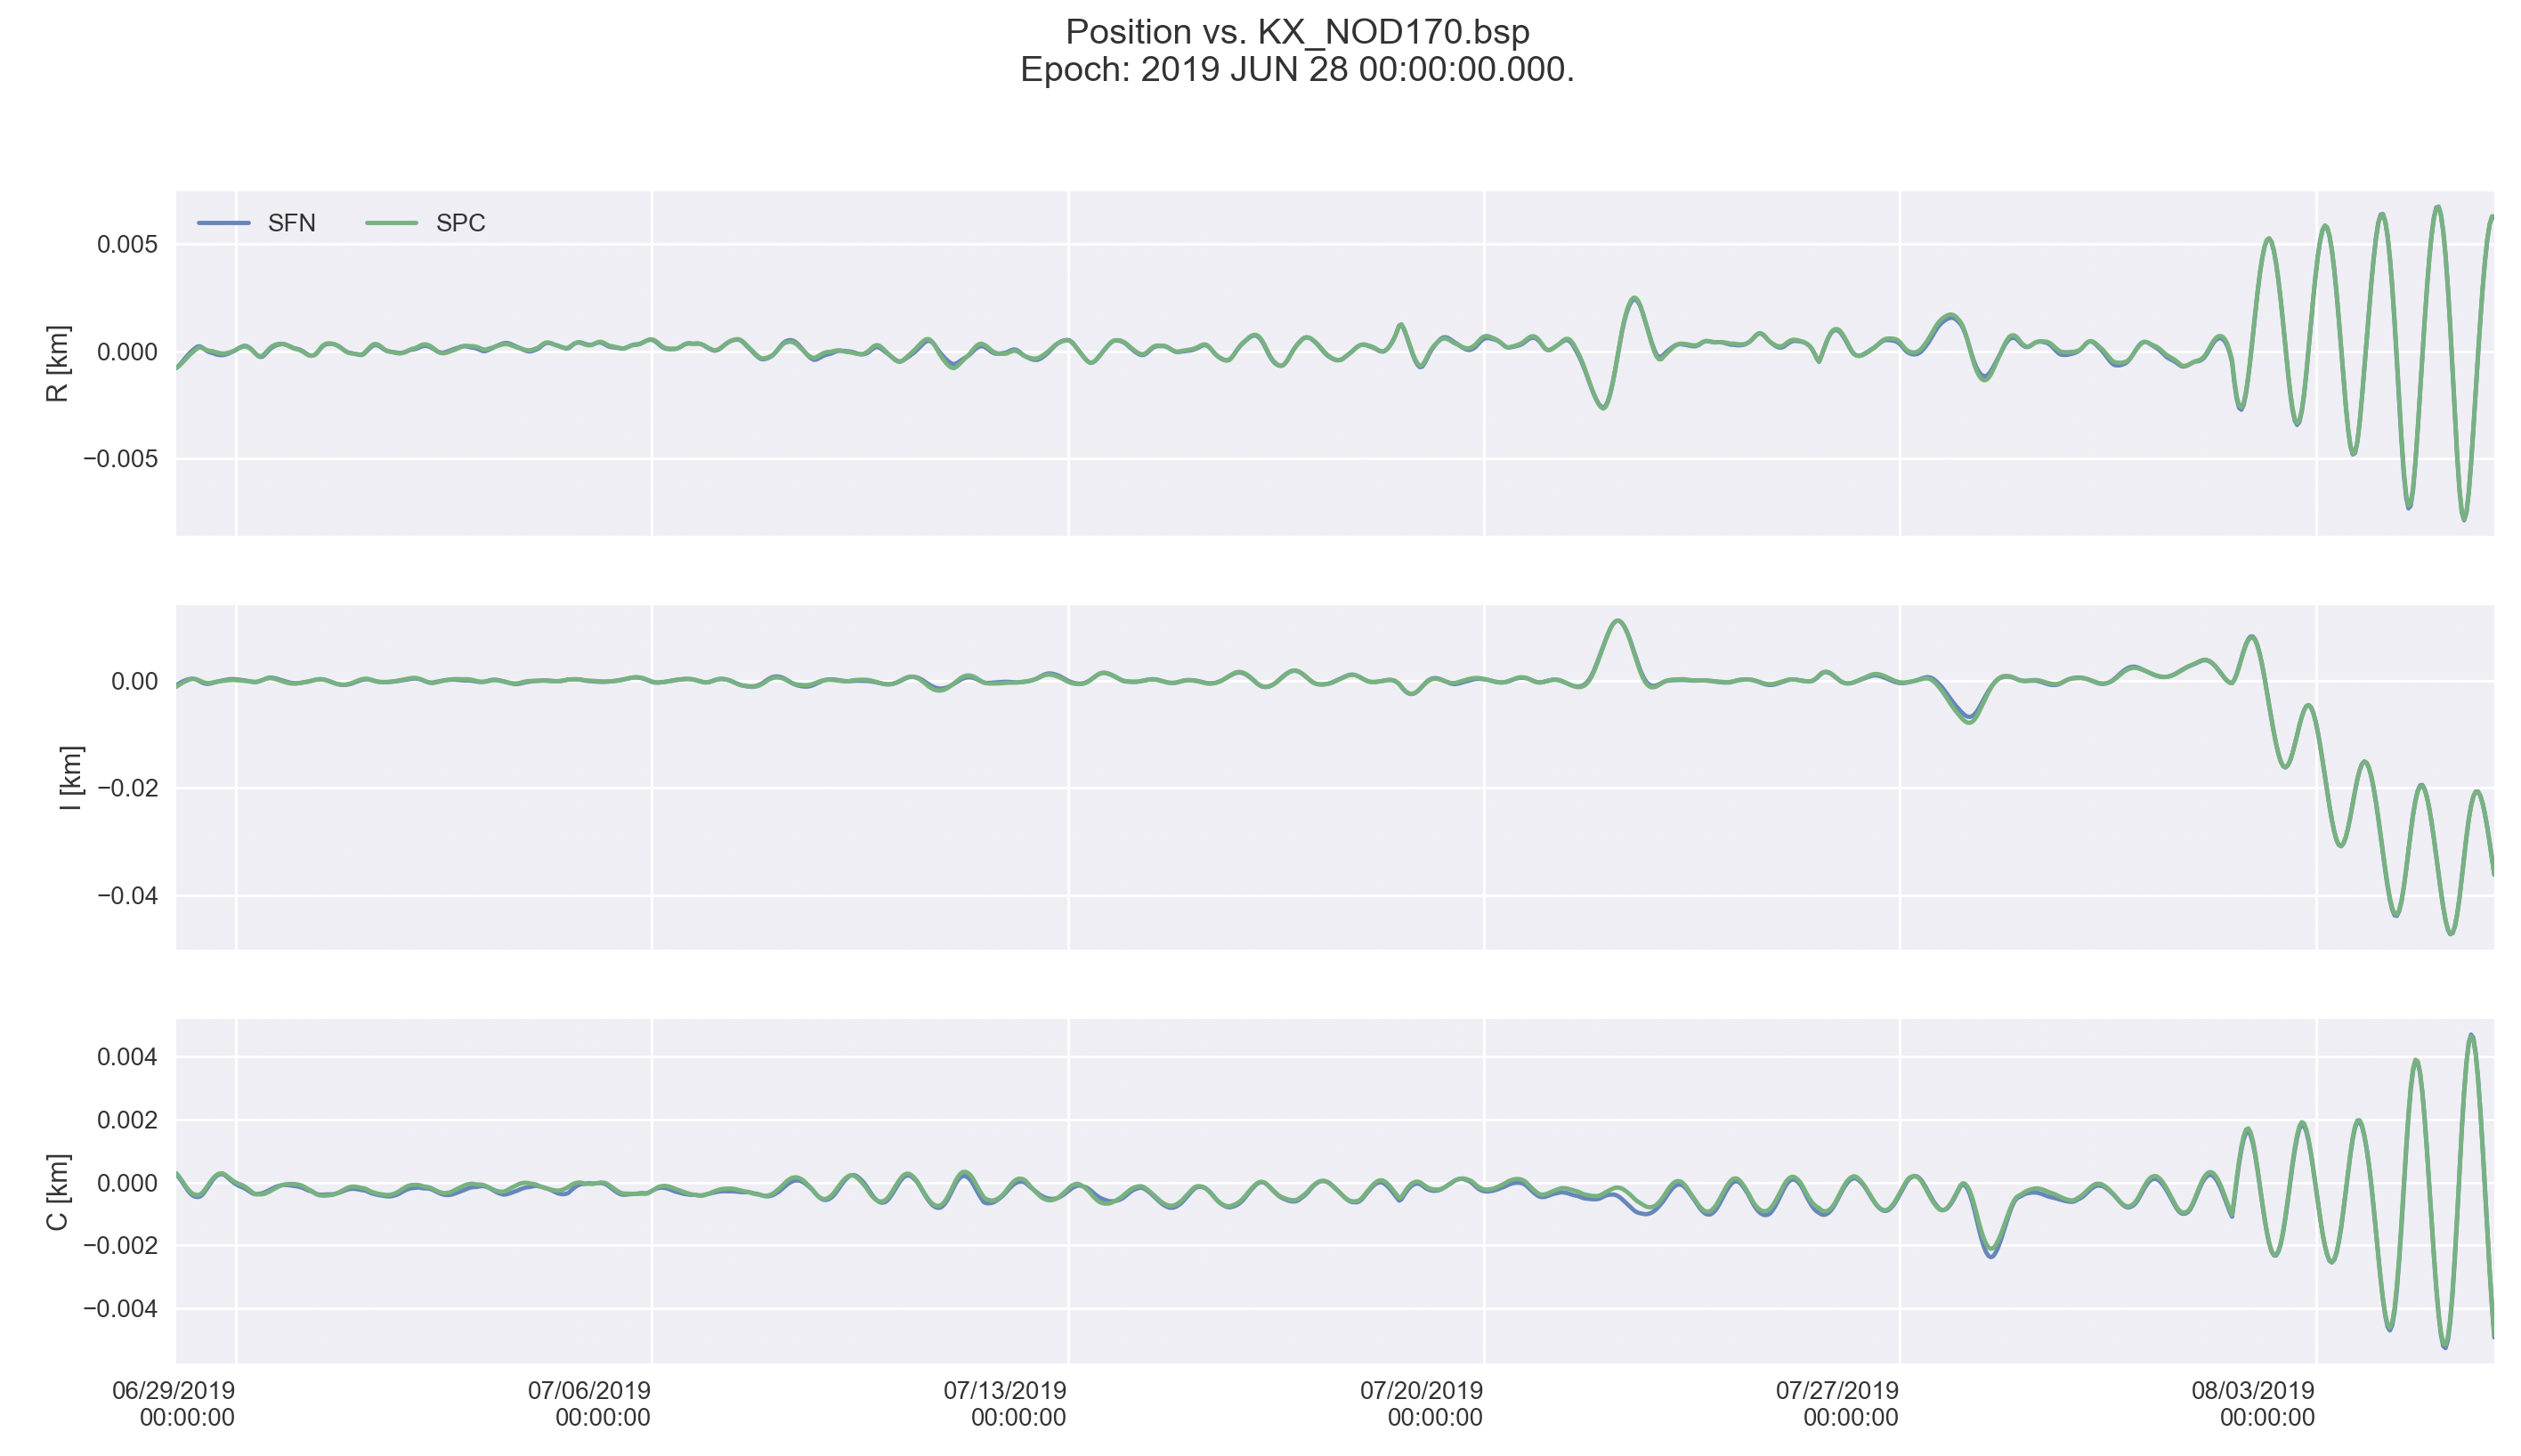
\includegraphics[width=\columnwidth]{orbitb_pfig.png}
    \caption{Trajectory position differences in the Bennu radial, in-track, cross-track (RIC) frame during Orbital B.  The comparison is between an orbit determination solution which uses SFN as the source of surface feature observations and the official orbit determination solution produced by KinetX which uses SPC as the source of surface feature observations.}
    \label{fig:obpos}
\end{figure}
\begin{figure}[h]
	\centering
	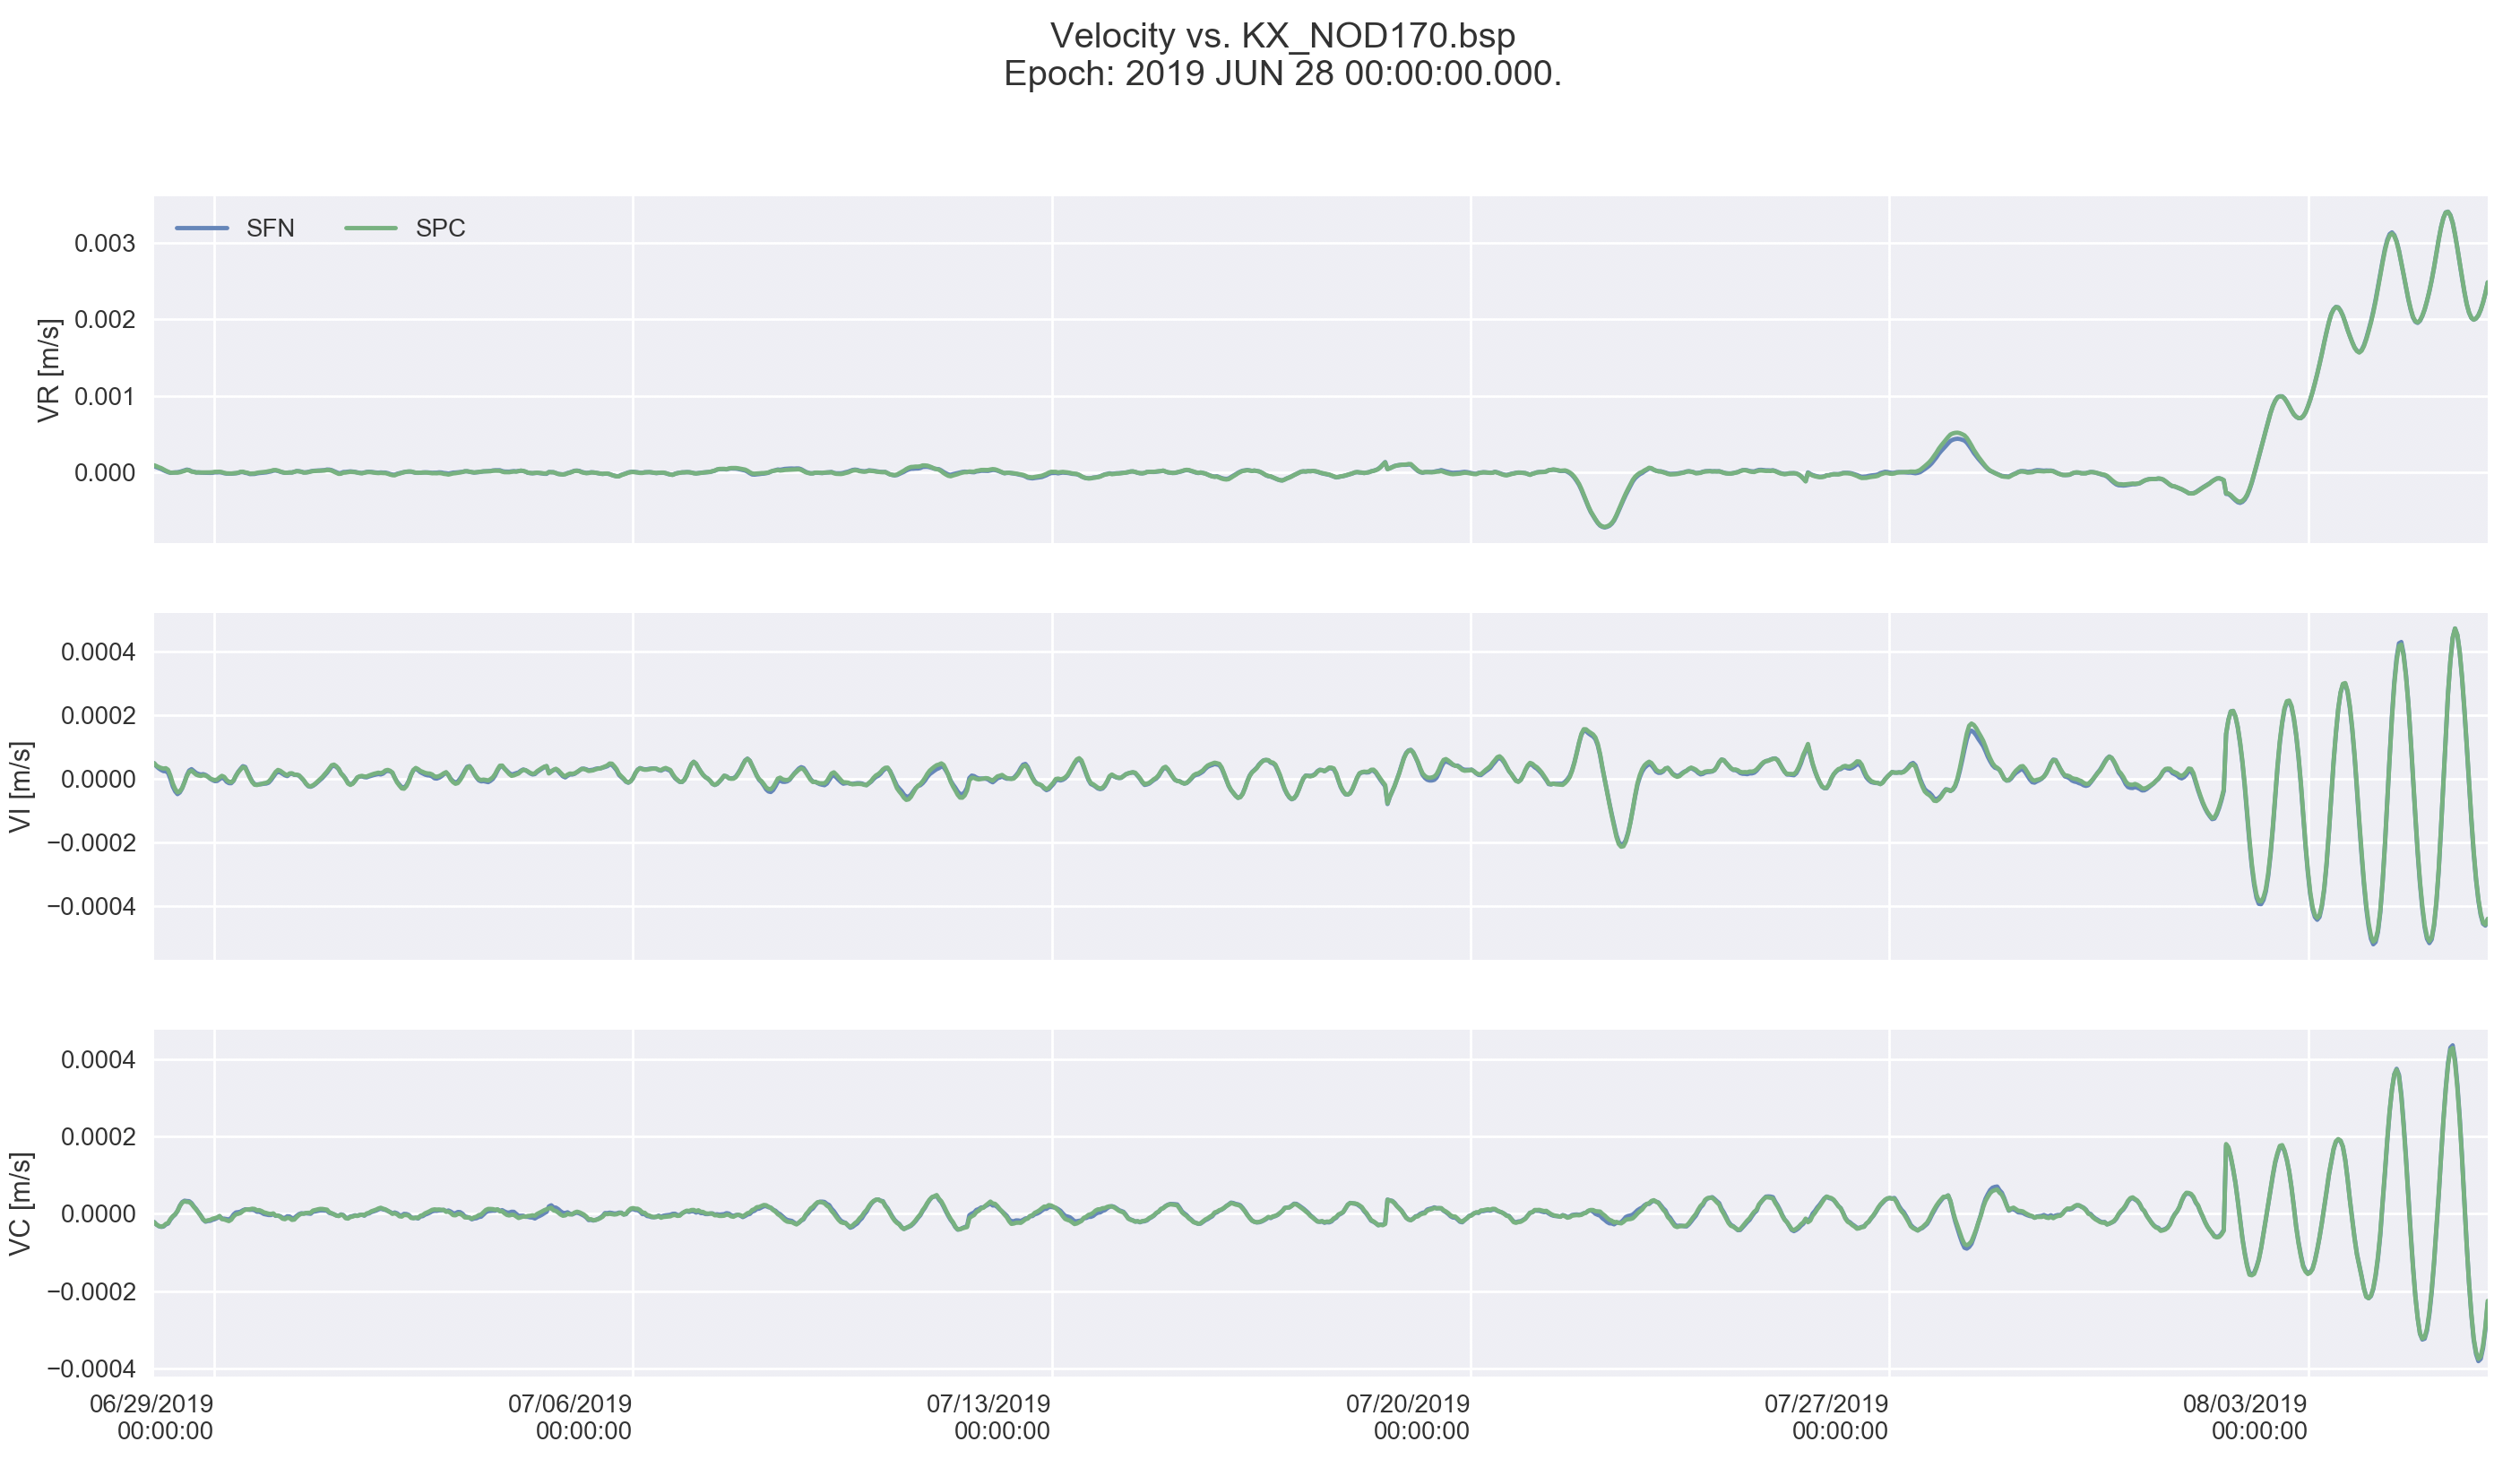
\includegraphics[width=\columnwidth]{orbitb_vfig.png}
    \caption{Trajectory velocity differences in the Bennu radial, in-track, cross-track (RIC) frame during Orbital B.  The comparison is between an orbit determination solution which uses SFN as the source of surface feature observations and the official orbit determination solution produced by KinetX which uses SPC as the source of surface feature observations.}
    \label{fig:obvel}
\end{figure}

As with Orbital A, the trajectories from the SFN and SPC processing match both each other and the KinetX solution quite closely over the period of time when observations were collected, as seen in Figs.~\ref{fig:obpos} and \ref{fig:obvel}.  The oscillations seen at the end of the arcs are again due to the ``data cutoff'', at which point no further data are included in the solution and the spacecraft state is base purely on dynamics integration.  This was done to evaluate the prediction performance of each technique.  The SFN data produce a very similar orbit to that estimated using the SPC data, again indicating that the method is working at least as well as SPC even in a different Orbital regime.

\textbf{OpNav Post-fit Residuals:}
Fig.~\ref{fig:obsfn} shows the post-fit residuals of the GIANT SFN observation in the GEODYN OD solution, and Fig.~\ref{fig:obspc} shows the same but for the SPC Residuals.  The post-fit residuals are once again similar as should be expected since the fit trajectories are similar.
\begin{figure}[htbp]
	\centering
	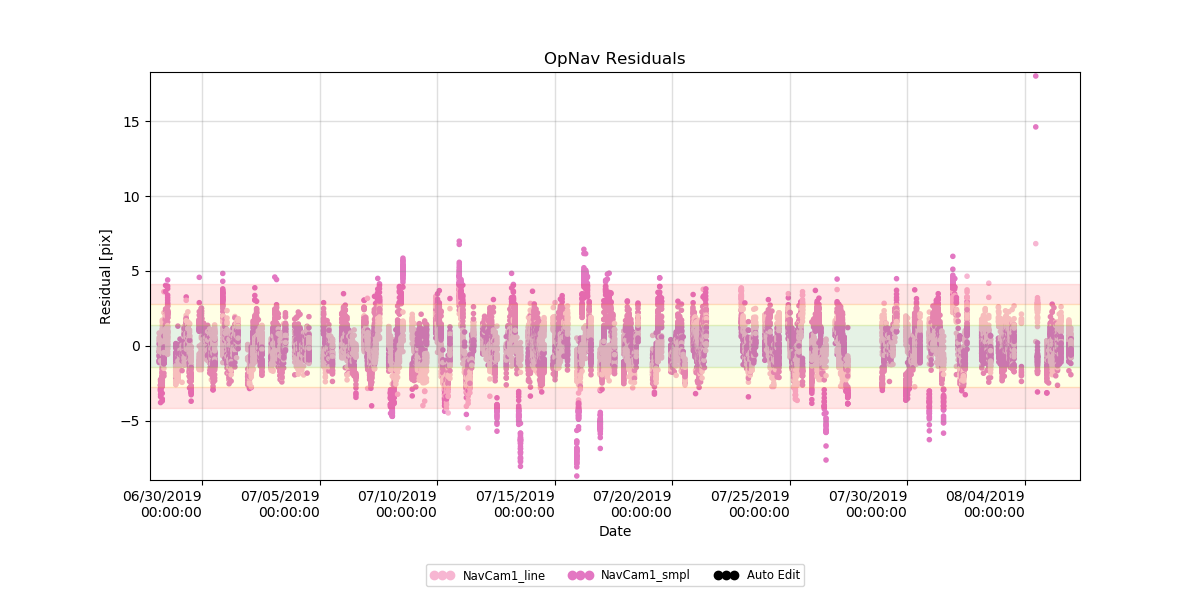
\includegraphics[width=\columnwidth]{orbitb_sfn.png}
    \caption{Post fit surface feature navigation residuals from GEODYN using GIANT SFN as the source of surface feature observation in Orbital B.}
    \label{fig:obsfn}
\end{figure}
\begin{figure}[htbp]
	\centering
	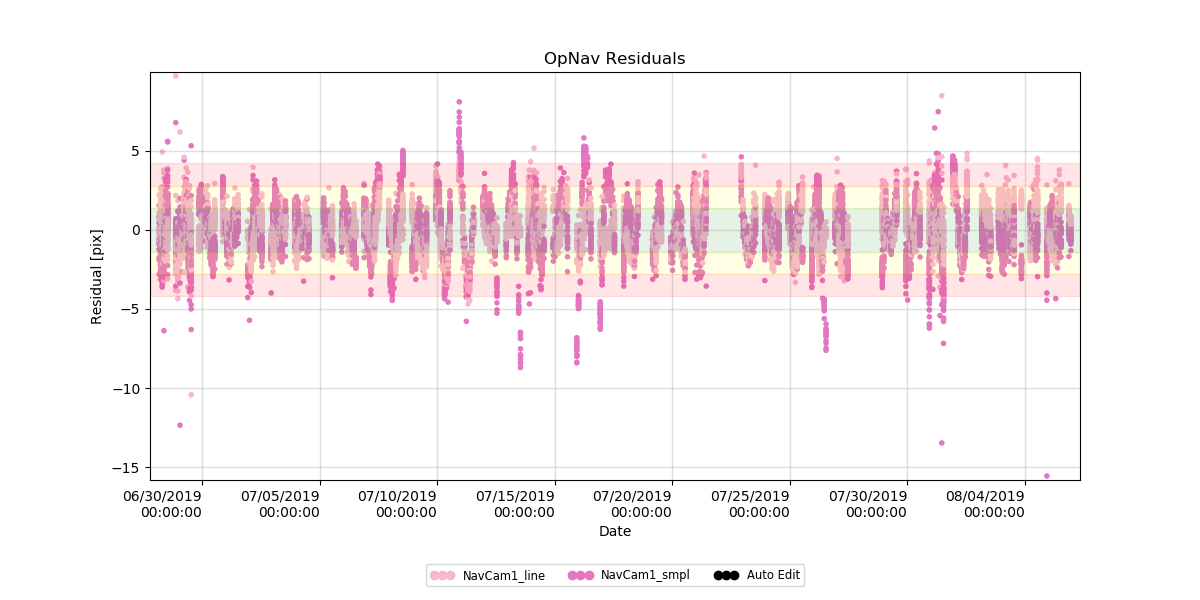
\includegraphics[width=\columnwidth]{orbitb_spc.png}
    \caption{Post fit surface feature navigation residuals from GEODYN using SPC as the source of surface feature observation in Orbital B.}
    \label{fig:obspc}
\end{figure}
% ====================================================
%     Conclusion
% ====================================================
\section*{Conclusions and Future Work}
The results from the Orbital A and Orbital B processing using SFN show extremely similar performance to SPC, the current state-of-the-art approach.  The final estimated trajectories differed by less than a meter throughout the entire observation period used.  This is a promising indication that continued development could yield valuable capabilities for future small body exploration missions.  Development and analysis will continue for this method, using navigation images from the OSIRIS-REx mission.

As discussed earlier, this method is only used for landmark identification using pre-constructed maplet topographies.  Due to this fact, we needed to use maplet topography generated by SPC.  SPC does not make full use of shadow information in the generation of maplets which leads to SPC underestimating heights/depths of boulders/craters, causing the entire maplet to be flattened.  This means that using our new method to predict shadows with these maplets can result in physically inaccurate shadows, degrading the SFN solutions, leading to more favorable conditions for SPC.  Despite this the performance between the two techniques is very similar, and in the future, we hope to take the principals of the SPC shape modeling techniques and combine them with new techniques to obtain structure from shadow to better estimate the terrain for predicting shadows, which should allow for more effective application of the SFN technique, and hopefully even better performance. 

% ====================================================
%     Acknowledgments
% ====================================================
\section*{Acknowledgments}
The authors are grateful to the entire OSIRIS-REx Team for making the encounter with Bennu possible.
They would also like to thank Cat Wolner for her help in preparing this manuscript.
This material is based upon work supported by NASA under Contracts NNM10AA11C and NNG13FC02C issued through the New Frontiers Program. 

% ====================================================
%     References
% ====================================================
\vspace{3pt}
\bibliographystyle{ieeetr}
\titleformat{\section}[runin]{\normalsize\bfseries}{\thesection}{0em}{\addperiod}
{\footnotesize \bibliography{references}}

% ====================================================
%     Additional Figures
% ====================================================


\end{document}
